% !TEX TS-program = pdflatex
% !TEX encoding = UTF-8 Unicode

% This is a simple template for a LaTeX document using the "article" class.
% See "book", "report", "letter" for other types of document.

\documentclass[11pt]{article} % use larger type; default would be 10pt

\usepackage[utf8]{inputenc} % set input encoding (not needed with XeLaTeX)

%%% Examples of Article customizations
% These packages are optional, depending whether you want the features they provide.
% See the LaTeX Companion or other references for full information.

%%% PAGE DIMENSIONS
\usepackage{geometry} % to change the page dimensions
\geometry{a4paper} % or letterpaper (US) or a5paper or....
% \geometry{margin=2in} % for example, change the margins to 2 inches all round
% \geometry{landscape} % set up the page for landscape
%   read geometry.pdf for detailed page layout information

\usepackage{graphicx} % support the \includegraphics command and options

% \usepackage[parfill]{parskip} % Activate to begin paragraphs with an empty line rather than an indent

%%% PACKAGES
\usepackage{booktabs} % for much better looking tables
\usepackage{array} % for better arrays (eg matrices) in maths
\usepackage{paralist} % very flexible & customisable lists (eg. enumerate/itemize, etc.)
\usepackage{verbatim} % adds environment for commenting out blocks of text & for better verbatim
\usepackage{subfig} % make it possible to include more than one captioned figure/table in a single float
% These packages are all incorporated in the memoir class to one degree or another...

%%% HEADERS & FOOTERS
\usepackage{fancyhdr} % This should be set AFTER setting up the page geometry
\pagestyle{fancy} % options: empty , plain , fancy
\renewcommand{\headrulewidth}{0pt} % customise the layout...
\lhead{}\chead{}\rhead{}
\lfoot{}\cfoot{\thepage}\rfoot{}

%%% SECTION TITLE APPEARANCE
\usepackage{sectsty}


\allsectionsfont{\sffamily\mdseries\upshape} % (See the fntguide.pdf for font help)
% (This matches ConTeXt defaults)

%%% ToC (table of contents) APPEARANCE
\usepackage[nottoc,notlof,notlot]{tocbibind} % Put the bibliography in the ToC
\usepackage[titles,subfigure]{tocloft} % Alter the style of the Table of Contents
\renewcommand{\cftsecfont}{\rmfamily\mdseries\upshape}
\renewcommand{\cftsecpagefont}{\rmfamily\mdseries\upshape} % No bold!

%%% END Article customizations


\usepackage[bulgarian]{babel}
\usepackage{physics}
\usepackage{amsmath}
\usepackage{centernot}
\usepackage{url}
\usepackage{graphicx}
\graphicspath{ {.} }
\usepackage{amsfonts}
\usepackage{xcolor}
\usepackage{enumitem}
\usepackage{systeme}


%%% The "real" document content comes below...

\title{24. Определен интеграл. Дефиниция и свойства. Интегруемост на непрекъснати функции...}
\author{Play4u}
%\date{} % Activate to display a given date or no date (if empty),
         % otherwise the current date is printed
         

\newcommand{\lrangle}[1]{\left\langle #1 \right\rangle}

\newcommand{\oversetModels}[1]{\overset{#1}{\models}}

\newcommand{\italicBold}[1]{\textbf{\emph{#1}}}

\newcommand{\definition}{\italicBold{Дефиниция: }}
\newcommand{\theorem}{\italicBold{Теорема: }}
\newcommand{\lemma}{\italicBold{Лема: }}
\newcommand{\proof}{\italicBold{Доказателство: }}
\newcommand{\statement}{\italicBold{Твърдение: }}
\newcommand{\source}{\italicBold{Източник: }}

\newcommand{\integral}[4]{\displaystyle \int_{#1}^{#2}#3\,#4}

\newcommand{\redText}[1]{\textcolor{red}{#1}}

\newcommand{\curlies}[1]{\{#1\}}
\newcommand{\overbar}[1]{\mkern 1.5mu\overline{\mkern-1.5mu#1\mkern-1.5mu}\mkern 1.5mu}

\newcommand{\enumNum}{\renewcommand{\theenumi}{\arabic{enumi}}}
\newcommand{\enumlet}{\renewcommand{\theenumi}{\alph{enumi}}} 

\begin{document}
\maketitle

\italicBold{Конспект: } Да се дефинират последователно: разбиване на интервал, диаметър на разбиване, риманова сума и риманов интеграл. Да се покаже, че всяка интегруема по Риман функция е ограничена.\\
Да се дефинират големи и малки суми на Дарбу. Да се установи, че при добавяне на нови точки в разбиването на интервала, големите суми на Дарбу не нарастват, а малките не намаляват(желателно е да се направи чертеж).\\
Да се долаже, че дадена функция е интегруема по Риман т.с.т.к. за всяко $\epsilon > 0$ съществуват голяма сума на Дарбу $S$ и малка сума на Дарбу $s$ такива, че $S-s < \epsilon$. Като се използва тази теорема и теоремата на Кантор, според която всяка непрекъсната функция в краен и затворен интервал е равномерно непрекъсната, да се докаже, че всяка непрекъсната функция вкраен и затворен интервал е интегруема по Риман. Да се изброят(\textit{без доказателство}) основните свойства на Римановия интеграл. Като се приложи свойството за интегриране на неравенства и теоремата, че всяка непрекъсната функция приема всички стойности между максимума и минимума си, да се докаже, че ако $f$ е непрекъсната в $[a,b]$, то съществува $c \in [a,b]$ така, че \\
\centerline{$\displaystyle\int_{b}^{a}f(x)\,dx=f(c)(b-a)$}.
Да се докаже теоремата на Нютон-Лайбниц, т.е. ако $f$ е непрекъсната в $[a,b]$, то за всяко $x \in [a,b]$\\
\centerline{$\displaystyle\frac{d}{dx}\integral{a}{x}{f(t)}{dt}=f(x)$;}
да се покаже как теоремата се използва за изчисляване на определен интеграл.

\section{Определени интеграли}

\definition Разбиване на интеграл: Всяка крайна система от точки $x_{0}, x_{1},...,x_{n}$, такива че $a = x_{0} < x_{1} < ...< x_{n} = b$ ще наричаме \textit{разбиване} на интервала $[a,b]$. Разбиванията ще означаваме с $\tau$, а точките на разбиването ще наричаме \textit{деляюи точки}. \\\par

\definition Диаметър на разбиване ще наричаме числото:\\
\centerline{$d(\tau)=\underset{1\leq i\leq n}{max}(x_{i}-x_{i-1})$.}\\\par

\definition Римановата сума за функцията $f(x)$, съотвестваща на разбиването на $\tau$ на интервала $[a,b]$ и избраните междинни точки $\curlies{\xi^{n}_{i=1}}$, се определя с формулата\\
\centerline{$R(f,\tau,\curlies{\xi_{i}}^{n}_{i=1})=\displaystyle\sum_{i=1}^{n}f(\xi_{i})(x_{i}-x_{i-1})$.}\\\par

\definition Риманов интеграл: Ще казваме, че числото $I$ е граница на римановите суми $R_{r}$ на $f$ в $[a,b]$ при $d(\tau) \to 0$(записваме $I = \lim_{d(\tau)\to 0}R_{\tau}$), ако за всяко $\epsilon > 0$ съществува $\delta > 0$ такова, че за всяко разбиване $\tau$ на $[a,b]$ с диаметър $d(\tau)<\delta$, имаме \\
\centerline{$R_{\tau}-I < \epsilon$}
(при произволен избор на междинните точки.)\par
Всяка функция $f$ за която съществува така дефинираната граница на римановите суми, ще наричаме \textit{интегруема} в интервала $[a,b]$. Границата $I$ се нарича \textit{определен интеграл} от функцията $f$ в интервала $[a,b]$ и се бележи с \\
\centerline{$I = \integral{a}{b}{f(x)}{dx}$. \t (Четем: интеграл от $a$ до $b$ от $f(x)dx$)}\\\par

\theorem Да се покаже, че всяка интегруема по Риман функция е ограничена:\\
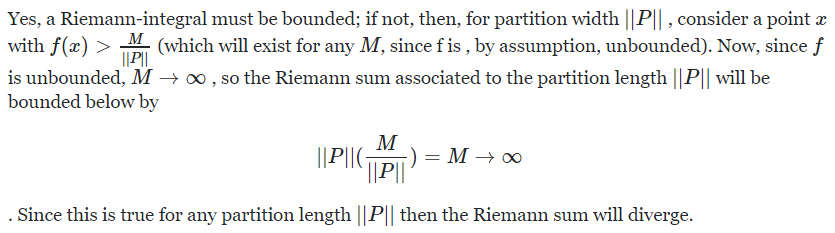
\includegraphics[scale=0.85]{RiemannBounded.png}

\definition Големи и малки суми на Дарбу: Нека предположим, че функцията $f(x)$ е ограничена в интервала $[a,b]$ и нека е зададено разбиване $\tau: = a=x_{0}<x_{1}<...<x_{n}=b$ на този интервал. Да означим с $M_{i}$, съответно с $m_{i}$, точната горна и точната долна граница на стойностите на $f(x)$ в интервала $[x_{i-1},x_{n}]$. Да разгледаме изразите:\\
\centerline{$S_{\tau} = \displaystyle \sum_{i=1}^{n}M_{i}(x_{i}-x_{i-1})$,}
\centerline{$s_{\tau} = \displaystyle \sum_{i=1}^{n}m_{i}(x_{i}-x_{i-1})$,}
които ще наричаме съответно голяма и малка \textit{сума на Дарбу}, съотвестващи на разбиването $\tau$.\\
На всяко разбиване $\tau$ съотвестват точно една малка и една голяма сума на Дарбу, за разлика от римановите суми, които са безбройно много. При това \\
\centerline{$s_{\tau}\leq R_{\tau}\leq S_{\tau}$}
независимо от междинните точки, използвани при получаването на $R_{\tau}$\\\par

\italicBold{Свойство: } Връзка между добавянето на нови точки в разбиването на интервала и сумите на Дарбу:\\
При добавяне на произволен брой точки към дадено разбиване, новата малка сума на Дарбу ще бъде по-голяма от старата, а новата голяма сума на Дарбу ще бъде по-малка от старата (с други думи със увеличаването на броя точки сумите на Дарбу се приближават една към друга (разбира се не е важна бройката на точките, а това че разбиването с повече точки ще съдържа разбиването с по-малко точки))\\
Ще казваме, че разбиването $\tau'$ \textit{следва} от разбиването $\tau$($\tau' \succ \tau$), ако делящите точки на $\tau$ са делящи точки и на $\tau'$.
\proof Достатъчно е да се разгледа случая, когато $\tau'$ се получава от $\tau$ чрез добавяне на една деляща точка. Нека означим с $x_{0}, x_{1},...,x_{n}$ делящите точки на $\tau$ и нека освен тях $\tau'$ да съдържа и още една деляща точка $x'$, лежаща в интервала $(x_{i-1},x_{i})$.\par

Да означим с $M'$ и $M''$ точната горна граница на $f(x)$ съответно в интервалите $[x_{i-1}, x']$ и $[x', x_{i}]$. Очевидно числата $M'$ и $M''$ не надминават $M_{i}$. Да сравним за изразите $S_{\tau}$ и $S_{\tau'}$. Ясно е, че $S_{\tau'}$ се получава от $S_{\tau}$, като събираемото $M_{i}(x_{i}-x_{i-1})$ се замени с две нови събираеми $M'(x'-x_{i-1})+M''(x_{i}-x')$. Имаме обаче\\
\centerline{$M'(x'-x_{i-1})+M''(x_{i}-x')\leq M_{i}(x'-x_{i-1})+M_{i}(x_{i}-x')=M_{i}(x_{i}-x_{i-1})$}
и следователно $S_{\tau} \geq S_{\tau'}$. Неравенството за малките суми на Дарбу се доказва аналогично\\
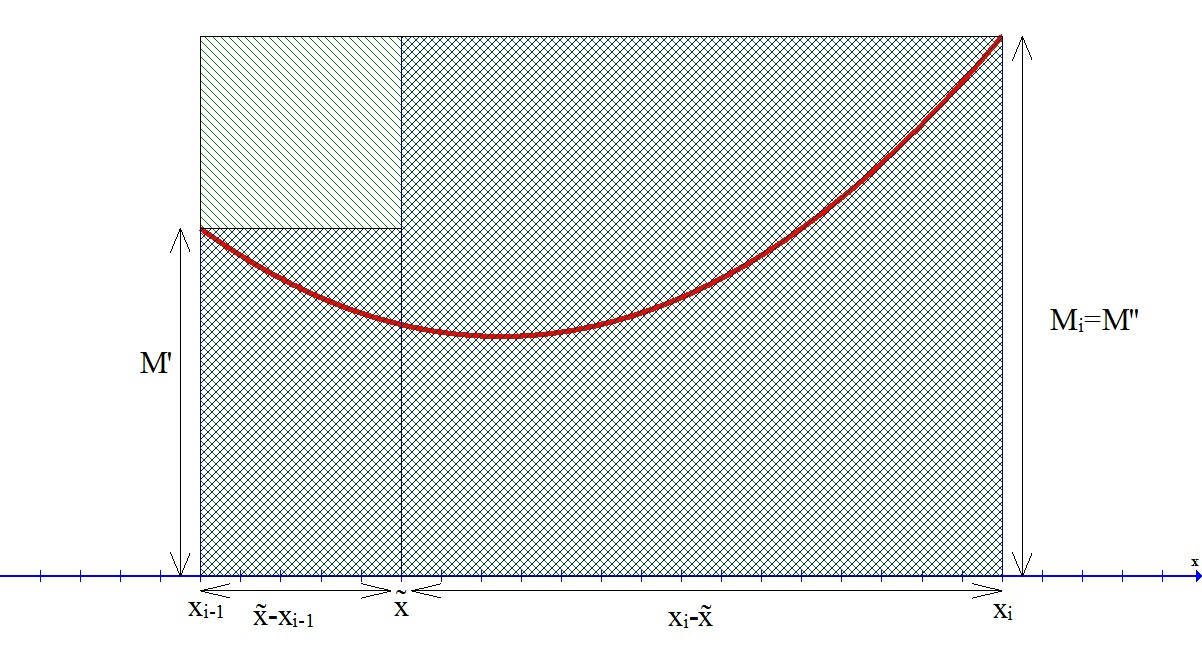
\includegraphics[scale=0.35]{Darbu.jpg}\\\par 

\theorem (\textbf{*})Функцията $f(x)$ е интергурема в $[a,b]$ (по Риман) тогава и само тогава, когато за всяко $\epsilon > 0$ съществуват разбивания $\tau_{1}$ и $\tau_{2}$ на интервала $[a,b]$, такива че \\
\centerline{$S_{\tau_1}-s_{\tau_2} < \epsilon$}
\proof \\
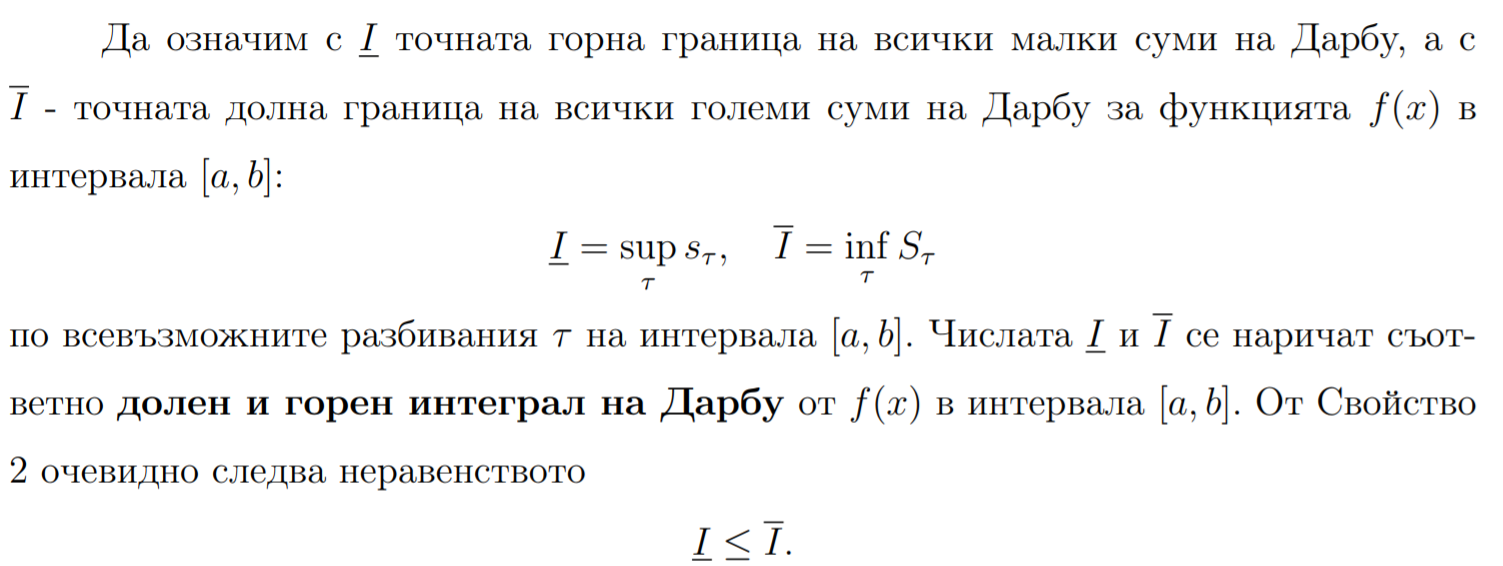
\includegraphics[scale=0.45]{UpperLowerDarbouxIntegral.png}
\\
Свойство 2: Всяка малка сума на Дарбу не надминава коя да е голяма сума на Дарбу\\
1.) Ако горното условие($S_{\tau_1}-s_{\tau_2}<\epsilon$) е изпълнено, то от неравентствата\\
\centerline{$s_{\tau_2} \leq \underline{I} \leq \bar{I} \leq S_{\tau_1}$}
следва, че $\bar{I}-\underline{I} < \epsilon$ за всяко $\epsilon > 0$. Следователно $\bar{I}=\underline{I}$.\\
2.) От определенията на точна долна и точна горна граница следва, че могат да се намерят разбивания $\tau_{1}, \tau_{2}$, така че\\
\centerline{$s_{\tau_2} > \underline{I}-\frac{\epsilon}{2}, \qquad S_{\tau_1} < \bar{I} + \frac{\epsilon}{2}$,}
откъдето, използвайки че $\underline{I} = \bar{I}$, веднага получаваме неравенството в условието\\\par

\theorem (За т-ма на (Кантор, разбивания) $\rightarrow$ интегруемост по Риман)
\source \path{http://info.fmi.shu-bg.net/skin/tfiles/vm2_019.pdf} (Теорема 3.) \\
\definition \textbf{Осцилация - $\omega(f)$: } Разликата между максималната и минималната стойност на фукция в даден интервал е нейното колебание (осцилация).\\
\proof Да фиксираме произволно $\epsilon > 0$. Ако функцията $f(x)$ е непрекъсната в интервала $[a,b]$, теоремата на Кантор и теорема \textbf{(*)} следва, че съществува $\delta > 0$ такова, че във всеки подинтеграл на $[a,b]$ с дължина по малка от $\delta$ осцилацията$(\omega)$ на $f(x)$ да бъде по-малка от $\dfrac{\epsilon}{b-a}$. Сега за всяко разбиване $\tau : a = x_{0} < x_{1} < ... < x_{n} = b$ с $\sigma(\tau) < \delta$ ще имаме, че за осцилацията във всеки интервал $[x_{i-1}, x_{i}]$ е изпълнено $\omega_{i}(f) < \dfrac{\epsilon}{b-a}$. Оттук\\
\centerline{$S_{\tau}-s_{\tau}=\displaystyle \sum_{i=1}^{n}\omega_{i}(x_{i}-x_{i-1}) < \dfrac{\epsilon}{b-a}\sum_{i=1}^{n}(x_{i}-x_{i-1})=\epsilon$}\\
Сега твърдението следва директно от критерия на Дарбу.

\section{Свойства на Раймановите интеграли}
\subsection{Линейност}
Нека функциите $f(x)$ и $g(x)$ са интегруеми в интервала $[a,b]$ и $\lambda \in \mathbb{R}$. Тогава $f(x)+g(x)$ и $\lambda f(x)$ също са интегруеми и са в сила равенствата \\
\centerline{$\integral{a}{b}{(f(x)+g(x))}{dx}=\integral{a}{b}{f(x)}{dx}+\integral{a}{b}{g(x)}{dx}$,}
\centerline{$\integral{a}{b}{\lambda f(x)}{dx} = \lambda \integral{a}{b}{f(x)}{dx}$.}

\subsection{Позитивност}
Ако $f(x)$ е неотрицателна интегруема функция, то \\
\centerline{$\integral{a}{b}{f(x)}{dx} \geq 0$}

\italicBold{(Опционално?: )Следствие: }\\
Нека $f(x)$ и $g(x)$ са интегруеми в $[a,b]$ и $f(x)\leq g(x)$
за всяко $x \in [a,b]$. Тогава\\
\centerline{$\integral{a}{b}{f(x)}{dx} \leq \integral{a}{b}{g(x)}{dx}$.}

\subsection{Това неравенство(няма по добро име)}
Ако функцията $f(x)$ е интегруема в $[a,b]$, то $|f(x)|$ е също интегруема в този интервал и е в сила неравенството: \\
\centerline{$|\integral{a}{b}{f(x)}{dx}| \leq \integral{a}{b}{|f(x)|}{dx}$.}

\subsection{Адитивност}
Нека $c \in [a,b]$. Тогава $f$ е интегруема в $[a,b]$ т.с.т.к. $f$ е интегруема във всеки от интегралите $[a,c]$ и $[c,b]$. При това\\
\centerline{$\integral{a}{b}{f(x)}{dx}=\integral{a}{c}{f(x)}{dx} + \integral{c}{b}{f(x)}{dx}$}
всеки път, когато трите интеграла съществуват.

\italicBold{2.4'} Равенството от свойство 4 е изпълнено при произволно разпределение не $a, b$ и $c$.

\subsection{Първа теорема за средната стойност}
Нека функциите $f(x)$ и $g(x)$ са интегруеми в интервала $[a,b]$, като $g(x)$ не си мени знака. Да означим с $M$ и $m$ точната горна и точната долна граница на $f(x)$ в $[a,b]$. Тогава съществува число $\mu, m \leq \mu \leq M$, за което е изпълнено равенството\\
\centerline{$\integral{a}{b}{f(x)g(x)}{dx} = \mu \integral{a}{b}{g(x)}{dx}$}\\\par

Използвайки теоремата за междинни стойности за непрекъснати функции получаваме:
\italicBold{Следствие. }Ако функцията $f(x)$ е непрекъсната в $[a,b]$, то съществува $\xi \in [a,b]$, така че\\
\centerline{$\integral{a}{b}{f(x)g(x)}{dx} = f(\xi)\integral{a}{b}{g(x)}{dx}$.}
Ще отблежим, че теоремата се използва най-често в случая, кгоато $g(x) = 1$ - тогава горното следствие се записва във вида:\\
\centerline{$\integral{a}{b}{f(x)}{dx}=f(\xi)(b-a)$}

\subsection{Втора теорема за средната стойност}
Нека функцията $f(x)$ е монотонно намаляваща и неотрицателна в $[a,b]$, а $g(x)$ е интегруема. Тогава съществува точка $\xi \in [a,b]$, такава че\\
\centerline{$\integral{a}{b}{f(x)g(x)}{dx} = f(a)\integral{a}{\xi}{g(x)}{dx}$}

\section{Изчисляване на интеграл}
\theorem (На Нютон-Лайбниц: ) Нека функцията $f$ е непрекъсната в интервала $[a,b]$. Тогава функцията $F$ е диференцируема и е в сила равенството\\
\centerline{$F'(x)=f(x)$}
\proof Нека $x \in [a,b]$ и нека $h$ е толкова малко, че $x+h$ също принадлежи на $[a,b]$. Да образуваме диференчното частно\\
\centerline{$\displaystyle \frac{F(x+h)-F(x)}{h}=\frac{1}{h}(\integral{a}{x+h}{f(t)}{dt}-\integral{a}{x}{f(t)}{dt})=\frac{1}{h}\integral{x}{x+h}{f(t)}{dt}$.}

Тогава според Следствието на първата теорема за средната стойност съществува $\xi \in (x, x+h)(\xi \in (x+h,x) \text{ при } h<0)$ такова, че \\
\centerline{$\frac{F(x+h)-F(x)}{h}=f(\xi)$}.
Ако сега оставим $h$ да клони към нула, то $\xi$ ще клони към $x$. Като използваме още веднъж непрекъсността на $f(x)$, получаваме исканото твърдение.\\\par

\italicBold{Формула на Нютон-Лайбниц. } От горната теорема е ясно как неопределеният интеграл от една непрекъсната функция, т.е. нейните примитиви, могат да се изразят чрез определения интеграл от нея. Следващото твърдение показва, обратно, как може да бъде пресметнат определения интеграл от функцията, ако е известна някоя нейна примитивна.\par
\textit{Нека $f(x)$ е непрекъсната в $[a,b]$ и $\Phi(x)$ е произволна нейна примитивна. Тогава е изпълнена формулата}\\
\centerline{$\integral{a}{b}{f(x)}{dx} = \Phi(b) - \Phi(a)$.}

\italicBold{Следствие: } Ако функцията $f$ притежава непрекъсната първа производна в $[a,b]$, то е в сила равенството\\
\centerline{$\integral{a}{b}{f'(x)}{dx} = f(x)\Big|_a^b$}

\italicBold{Пример: } Имаме\\
\centerline{$\integral{0}{\pi}{sin\;x}{dx}=(-cos\;x)\big|_0^\pi=1-(-1)=2$} 
  
\end{document}





